This chapter explains the design and development method used to build VietFlood. The work follows a build-and-check approach common in software engineering: define scope, model the actors and workflows, design the system structure and data model, implement the prototype, and validate the result through end-to-end scenarios. The goal is not to run a controlled experiment. The goal is to produce a coherent prototype whose structure matches the responsibilities of reporting, review, and role-based access control \cite{bass2021softwareArchitecture}.

\section{Method Overview}

The project targets one specific part of flood response: turning scattered observations into structured reports that can be reviewed and tracked over time. VietFlood does not attempt to predict floods, dispatch resources, or replace official warning systems. The methodology therefore focuses on features that can be implemented and verified within a thesis prototype:
\begin{itemize}
    \item authentication and session handling;
    \item report submission with location fields and optional evidence;
    \item persistent storage of reports and evidence metadata;
    \item administrator review and status updates;
    \item relief-oriented reading views, including map-related screens;
    \item a minimal real-time channel for location sharing.
\end{itemize}

\section{Design Inputs and Constraints}

Requirements were derived from the intended workflow and the realities of mobile reporting during disruptive conditions. The system must accept short, incomplete, and sometimes noisy input, while still producing records that can be searched and compared. Constraints that shaped the method include limited development time, prototype-level testing, and the lack of validated field datasets.

\subsection{Functional Goals}

Requirements are grouped by the three roles implemented in the prototype:
\begin{itemize}
    \item \textbf{Citizen:} register/sign in, manage profile fields, create reports with address and coordinates, attach photo evidence, and view personal report history.
    \item \textbf{Relief:} browse report information and location-oriented views without changing report status.
    \item \textbf{Administrator:} review all reports, search/filter records, inspect evidence and reporter details, update report status, and manage user accounts.
\end{itemize}

Each report stores a short description, location fields (province, ward, address line, latitude/longitude), severity/urgency values, timestamps, and a review status. Status values are kept intentionally small in this thesis version: \texttt{pending}, \texttt{verified}, \texttt{resolved}, and \texttt{rejected}. This is enough to demonstrate review and follow-up without introducing a complex workflow engine.

\subsection{Quality and Operational Goals}

Several non-functional goals guided design choices:
\begin{itemize}
    \item \textbf{Separation of concerns:} authentication logic should not be mixed with report persistence and evidence handling.
    \item \textbf{Evidence storage outside the database:} images should be stored in a media platform, while the database keeps searchable metadata and report fields.
    \item \textbf{Repeatable runtime:} the system should run locally and in deployment using the same container-based configuration.
    \item \textbf{Simple boundaries:} service splits should be justified by responsibility, not by a desire to maximize the number of services.
\end{itemize}

\section{Role and Use-Case Modeling}

Actors were modeled first because they define who can perform each operation and what information each role should see. Use-case diagrams were used to keep the prototype scope clear and to avoid designing features that do not fit the stated responsibilities.

\subsection{Citizen Role}

The citizen actor represents a member of the public reporting an observed flood situation. The citizen workflow begins with registration or sign-in, then continues to report creation by entering a description, selecting location fields, attaching photos when available, and submitting the report. The mobile client can help by reading device location and by listing Vietnam administrative divisions to reduce inconsistent spelling.

\begin{figure}[htbp]
    \centering
    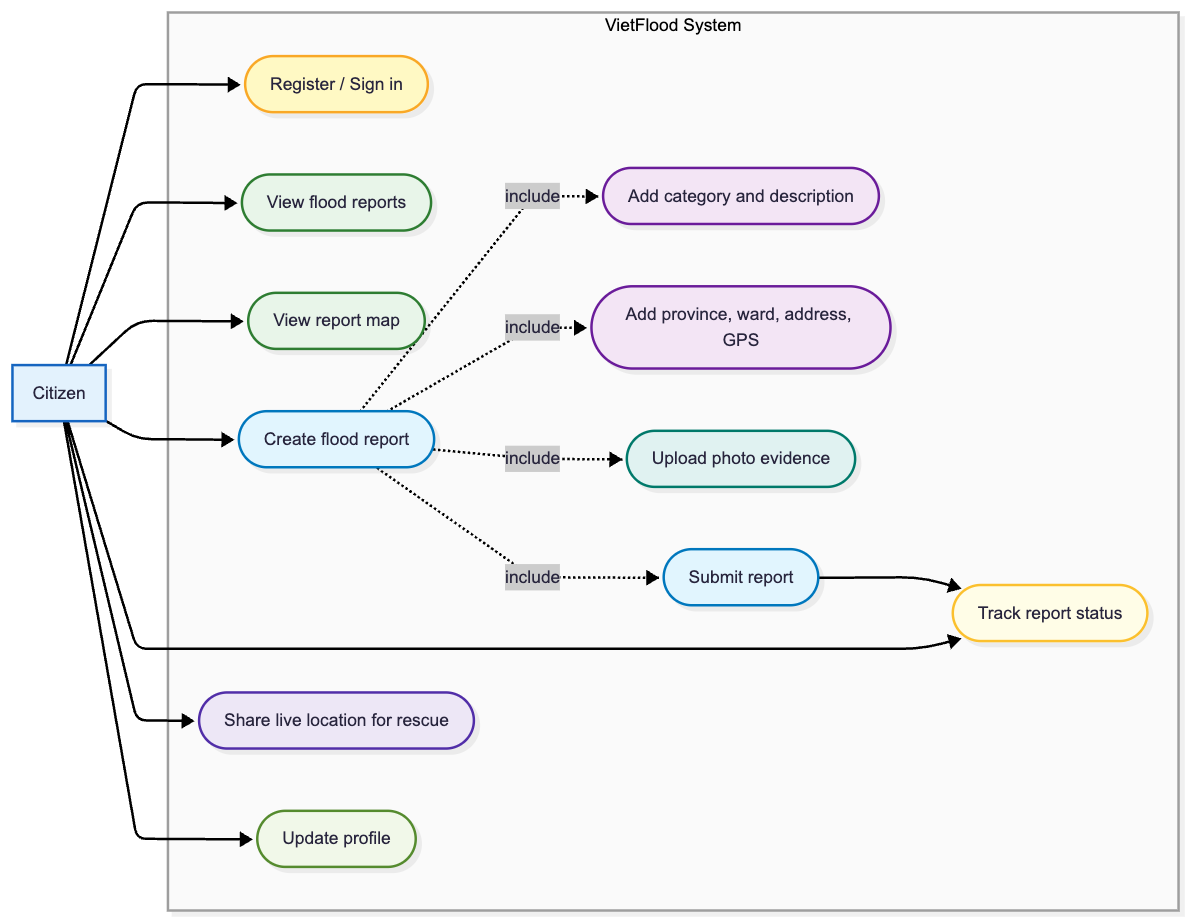
\includegraphics[width=0.74\linewidth,height=0.36\textheight,keepaspectratio]{images/figure3-1-citizen-use-case.png}
    \caption{Citizen capabilities supported by VietFlood (use case view).}
    \label{fig:method-citizen-usecase}
\end{figure}

\subsection{Relief Role}

The relief actor represents users who need situational awareness from submitted reports. In the prototype, the relief role can browse report lists, open details, and use map-related views. The relief role does not verify or reject reports. Keeping verification in the administrator workflow avoids conflicting status changes and keeps the trust signal (status) under one authority in this thesis scope.

\begin{figure}[htbp]
    \centering
    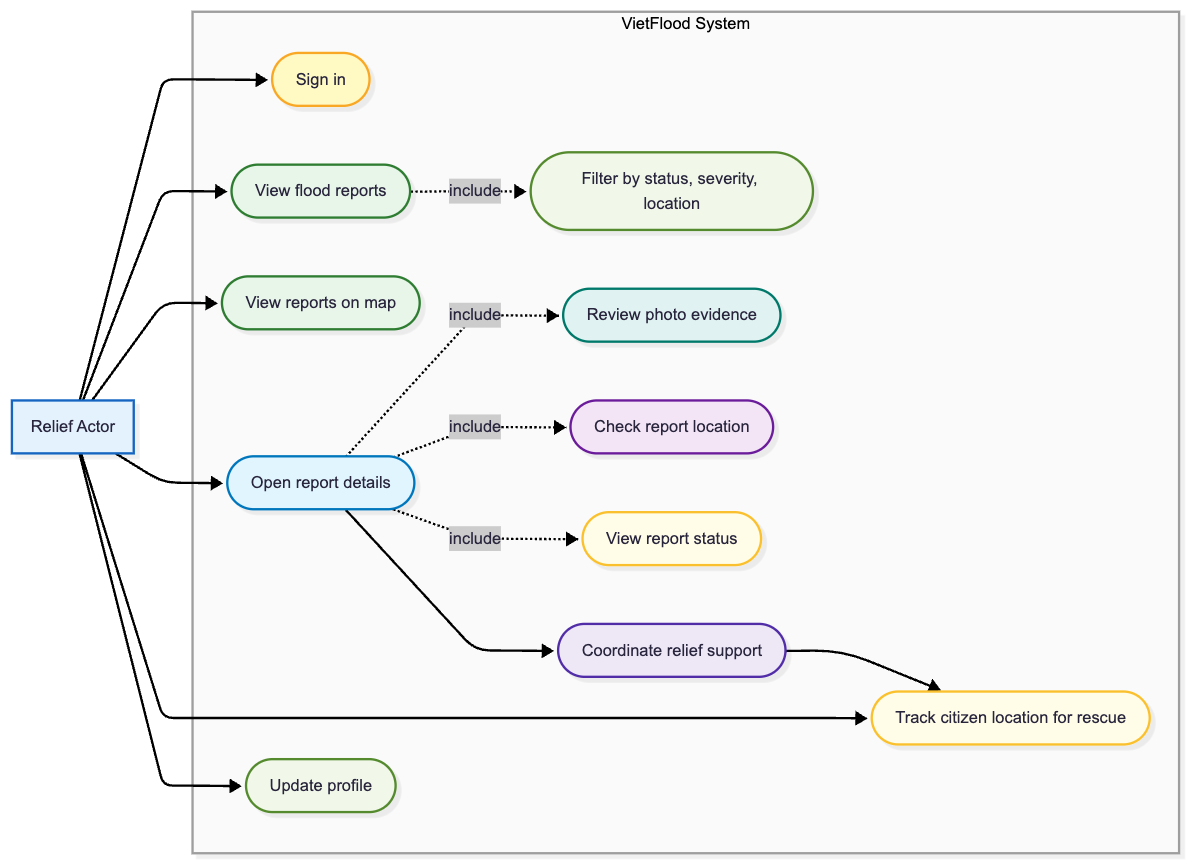
\includegraphics[width=0.74\linewidth,height=0.36\textheight,keepaspectratio]{images/figure3-2-relief-use-case.png}
    \caption{Relief browsing features supported by VietFlood (use case view).}
    \label{fig:method-relief-usecase}
\end{figure}

\subsection{Administrator Role}

The administrator actor uses the web dashboard to review incoming reports. The dashboard presents report fields, reporter details, evidence previews, and tools for filtering and searching. Administrator actions include changing status values and managing user records. The web client checks the current profile and role before showing administrator screens so a non-admin account cannot access the review workspace by direct URL navigation.

\begin{figure}[htbp]
    \centering
    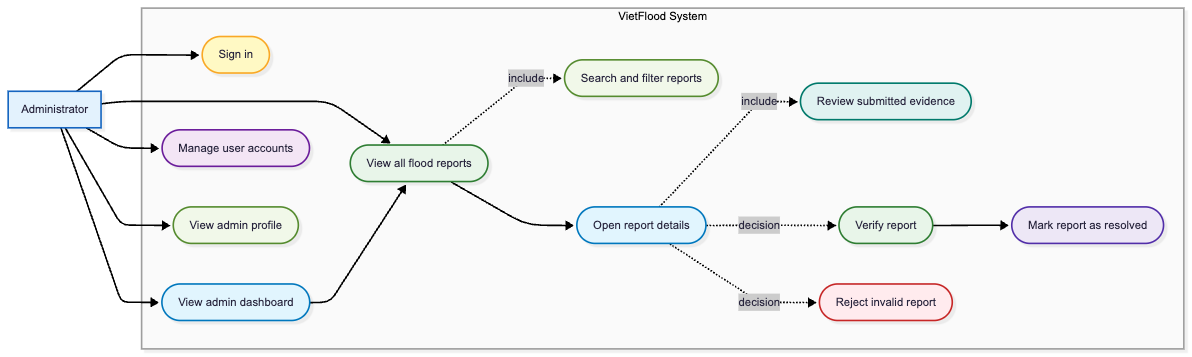
\includegraphics[width=0.74\linewidth,height=0.36\textheight,keepaspectratio]{images/figure3-3-admin-use-case.png}
    \caption{Administrator review and management features (use case view).}
    \label{fig:method-admin-usecase}
\end{figure}

\section{Development Materials and Tools}

Development work was organized into four code modules to keep responsibilities clear. The backend module contains the NestJS API gateway and internal services \cite{nestjsDocs,nestjsMicroservicesDocs}. The shared module (\texttt{vietflood\_common}) provides common infrastructure utilities. The mobile module contains the Expo React Native application \cite{expoDocs,reactNativeDocs}. The web module contains the Next.js administrator dashboard \cite{nextjsDocs}. Table~\ref{tab:method-tools} summarizes the main tools used.

\begin{table}[htbp]
\centering
\caption{Materials, tools, and runtime dependencies used during VietFlood development.}
\label{tab:method-tools}
\begin{tabular}{|>{\raggedright\arraybackslash}p{4cm}|>{\raggedright\arraybackslash}p{9cm}|}
\hline
\textbf{Area} & \textbf{Tools and purpose} \\
\hline
Backend & NestJS, TypeScript, TypeORM, PostgreSQL, RabbitMQ, Redis, Socket.IO, JWT, bcrypt. \\
\hline
Shared package & \texttt{vietflood\_common} for structured logging, Redis client setup, and Cloudinary file operations. \\
\hline
Mobile client & Expo, React Native, TypeScript, React Navigation, Redux Toolkit, image picking, secure token storage, device location, and Vietnam Provinces Open API. \\
\hline
Web dashboard & Next.js, React, TypeScript, Tailwind CSS, protected admin login, token refresh, report overview, search, filtering, evidence preview, and status update. \\
\hline
Runtime infrastructure & Docker, Docker Compose, PostgreSQL, Redis, RabbitMQ, Cloudinary, and Azure App Service configuration. \\
\hline
\end{tabular}
\end{table}

\section{Architecture Design Approach}

The system was designed as a small set of services rather than a single monolithic backend. The point of the service split is not complexity; it is ownership. Authentication and report persistence evolve differently and have different failure modes. Keeping them separate reduces accidental coupling and keeps code easier to reason about during iteration. At the same time, the number of services is kept low to avoid operational overhead that would not pay off at prototype scale \cite{fowlerLewis2014microservices,dragoni2017microservices,thones2015microservices}.

In VietFlood, the API gateway is the single public entry point. It handles HTTP routes and the Socket.IO channel exposed to clients. The authentication service owns registration, sign-in, token refresh, profile operations, and user management. The reports service owns report creation, listing, status updates, evidence metadata storage, and cache invalidation. Redis, RabbitMQ, PostgreSQL, and Cloudinary provide supporting infrastructure for caching, messaging, persistence, and evidence storage.

\begin{figure}[htbp]
    \centering
    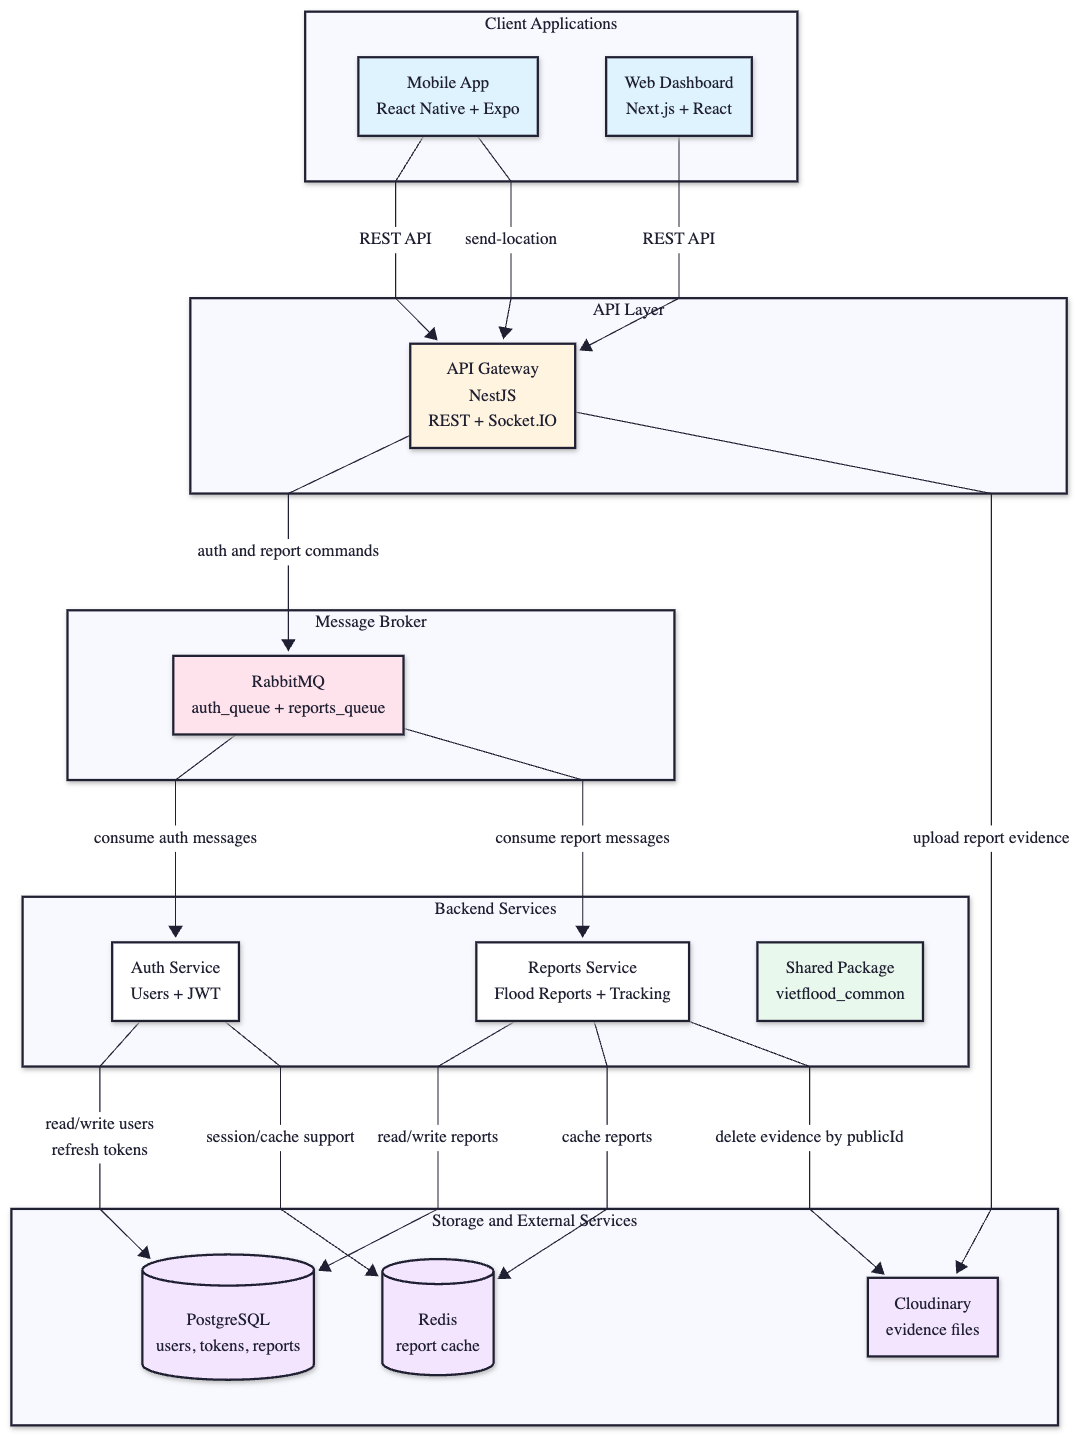
\includegraphics[width=1\linewidth,height=0.44\textheight,keepaspectratio]{images/figure3-4-system-architecture.png}
    \caption{System architecture overview of VietFlood components and their interactions.}
    \label{fig:method-system-architecture}
\end{figure}

\subsection{Gateway Interface Design}

The gateway exposes the REST interface consumed by both the mobile and web clients. Authentication routes are grouped under \texttt{/auth} and report routes under \texttt{/reports}. Report creation is implemented as a multipart upload; the gateway processes uploaded files, uploads evidence to Cloudinary, and then forwards the final report payload to the reports service. Centralizing evidence upload in the gateway avoids duplicating upload logic across services and keeps clients unaware of internal service boundaries.

The gateway also enforces JWT authentication and role checks. Citizen endpoints are scoped to personal report operations, broader report reading is available to relief and admin accounts, and administrator-only operations are protected separately.

\subsection{Service Messaging Design}

Internal service calls use RabbitMQ request--response messaging \cite{rabbitmqConfirmsDocs}. The gateway sends authentication commands to the auth service and report commands to the reports service. This makes the boundary explicit: the gateway does not directly access the database owned by the services, and each service can validate inputs and return controlled responses.

Messaging also makes troubleshooting more concrete during development. If a report creation fails, the failure can be localized to one of a small number of steps: request parsing, evidence upload, message transport, or service-side validation/persistence.

\section{Data Modeling Approach}

The data model was designed to support the report lifecycle while staying small enough to evolve during prototyping. PostgreSQL is used for persistence and TypeORM entities map application objects to relational tables \cite{typeormDocs}. The core tables are users and reports.

User records store identity fields (email, username, phone), a bcrypt-hashed password, role, basic profile information, and timestamps. Uniqueness constraints on email/username/phone prevent duplicate accounts.

Report records store a textual description, category values, administrative location fields (province, ward, address line), coordinates, urgency/severity values, timestamps, and a status field used for review. Evidence is stored as JSON metadata rather than raw bytes: each item includes a delivery URL and a Cloudinary public ID. This keeps media delivery out of the database while still making the report record self-contained for review \cite{postgresqlJsonDocs,cloudinaryUploadDocs}.

\begin{figure}[htbp]
    \centering
    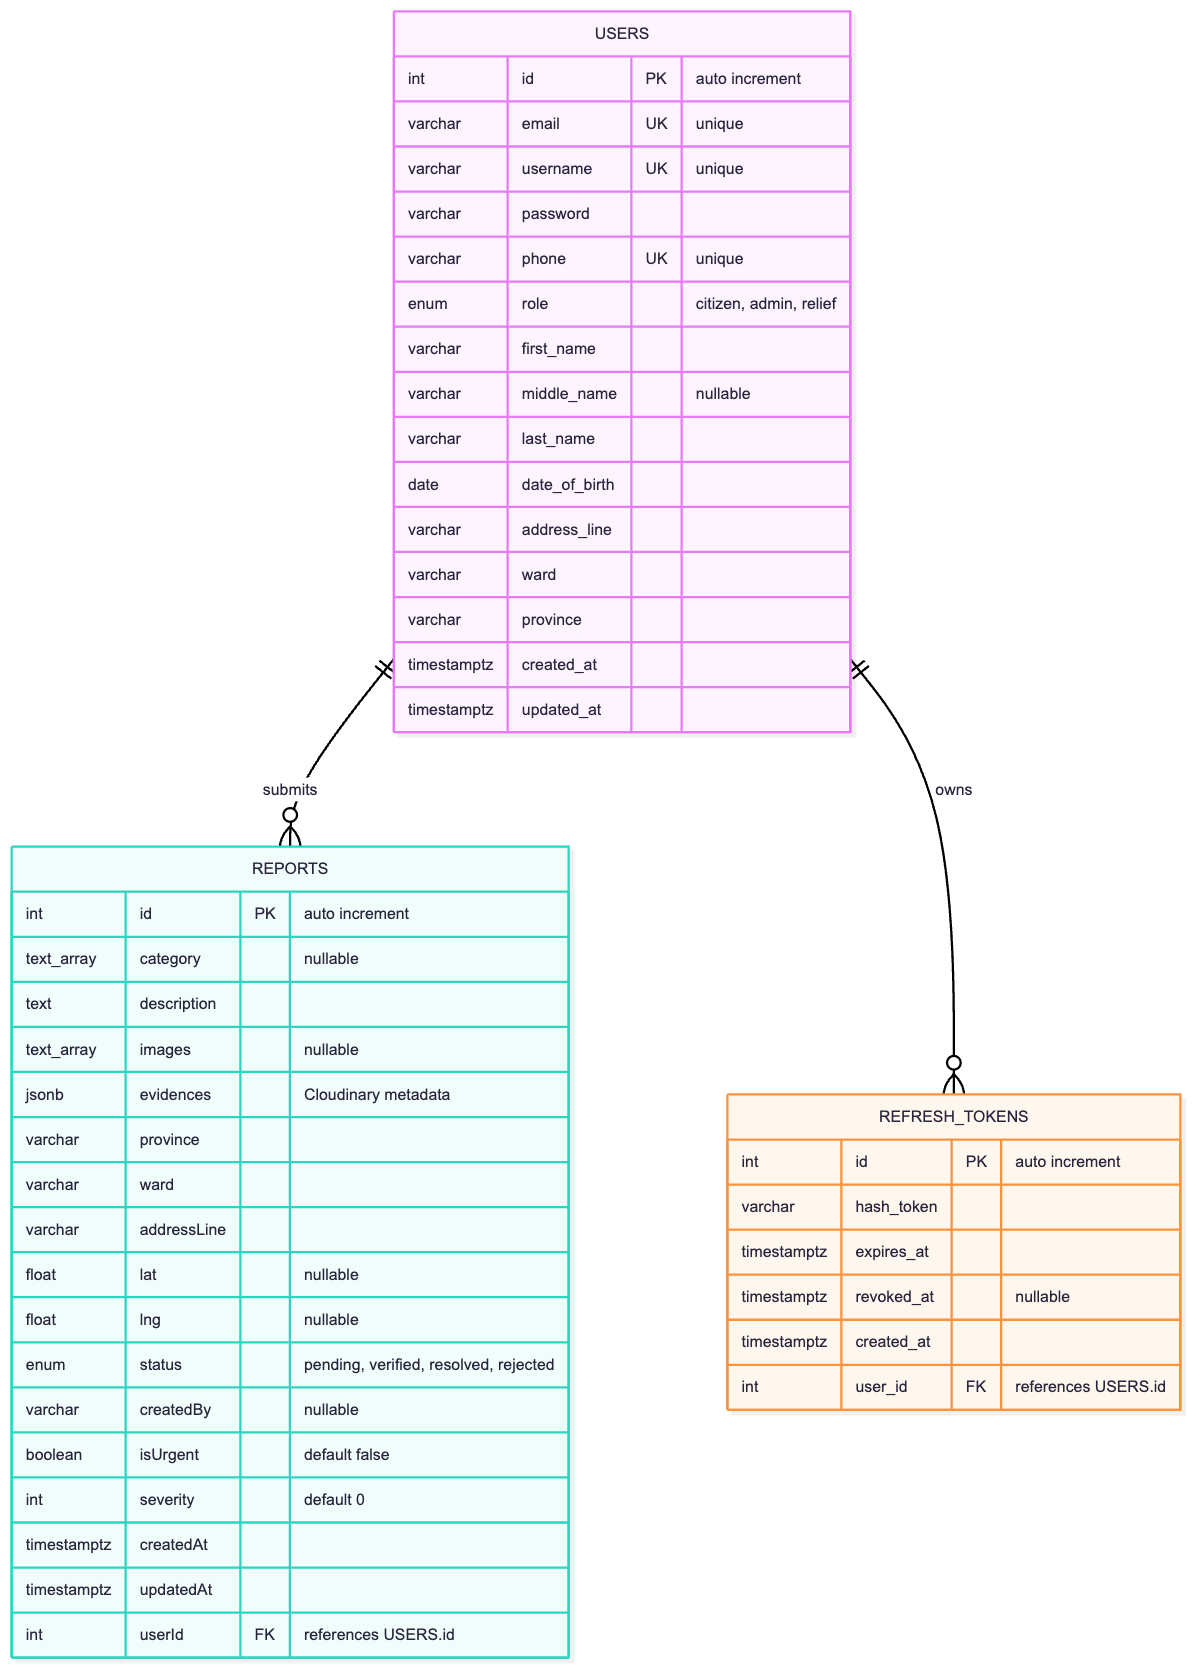
\includegraphics[width=0.9\linewidth,height=0.42\textheight,keepaspectratio]{images/figure3-5-database-schema.png}
    \caption{Prototype database schema showing the core entities and relationships.}
    \label{fig:method-database-schema}
\end{figure}

\subsection{Caching Approach}

Redis is used as a cache layer, not as the source of truth \cite{redisDocs}. The reports service writes a cached report entry after create/update operations and checks the cache before reading from PostgreSQL on lookups. When a report changes or is deleted, the corresponding cache entry is refreshed or removed. Cache scope is kept narrow on purpose to make invalidation behavior clear in a prototype setting.

\section{Workflow Specification}

Workflows were specified as sequences across the client, gateway, and internal services. The primary workflow is report creation. A citizen enters a description and location fields, optionally selects photo evidence, and submits the report from the mobile app. The gateway authenticates the request, uploads evidence to Cloudinary, and forwards the final payload to the reports service. The reports service persists the report and updates the cache.

\begin{figure}[htbp]
    \centering
    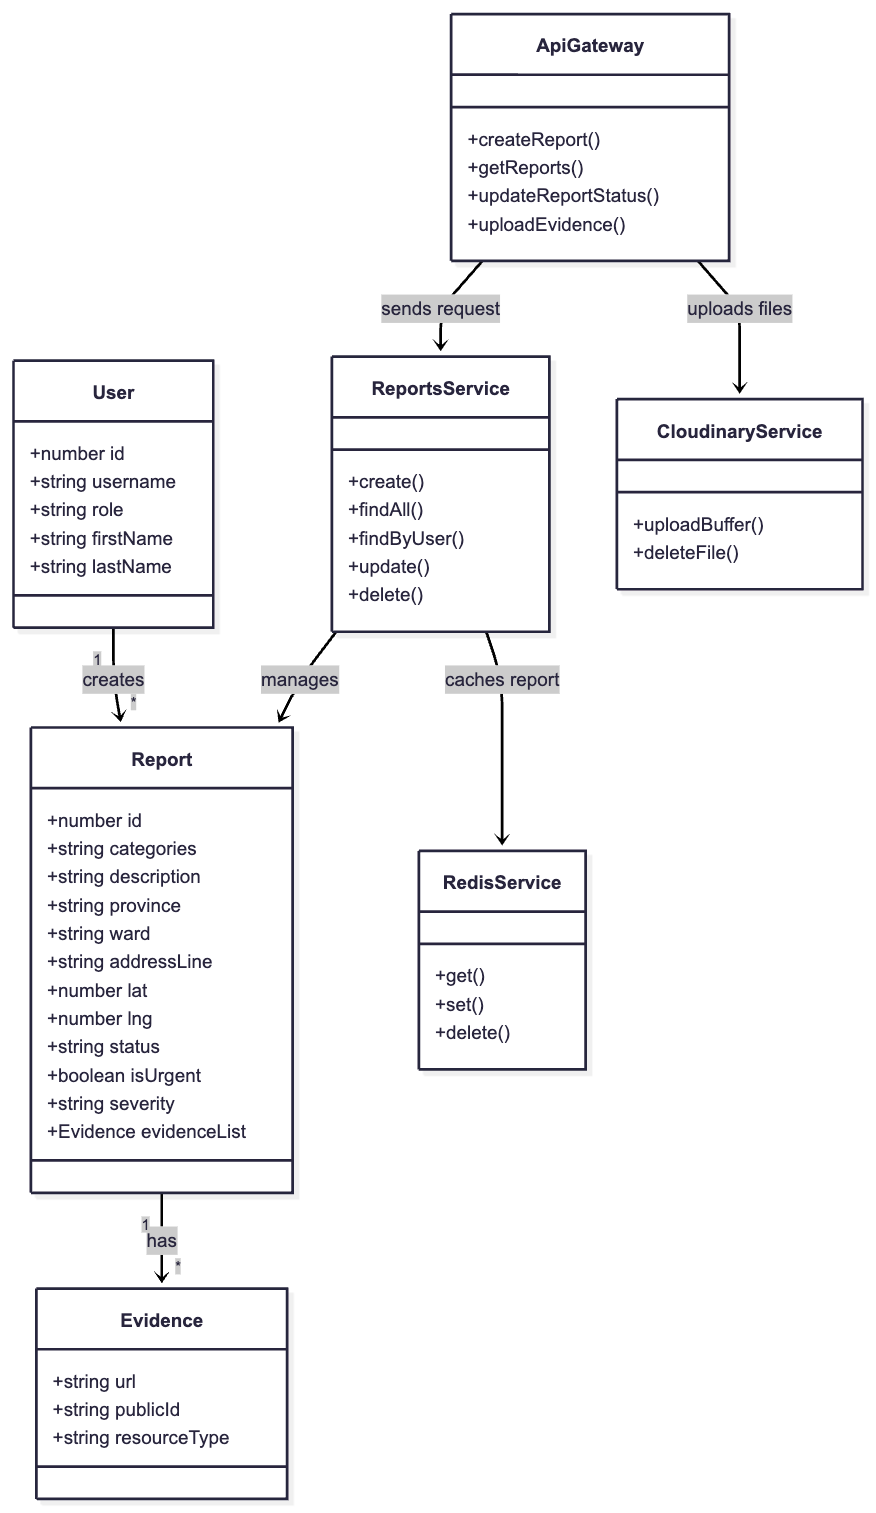
\includegraphics[width=0.9\linewidth,height=0.42\textheight,keepaspectratio]{images/figure3-6-report-class-diagram.png}
    \caption{Core data structures used in the report workflow.}
    \label{fig:method-report-class}
\end{figure}

\begin{figure}[htbp]
    \centering
    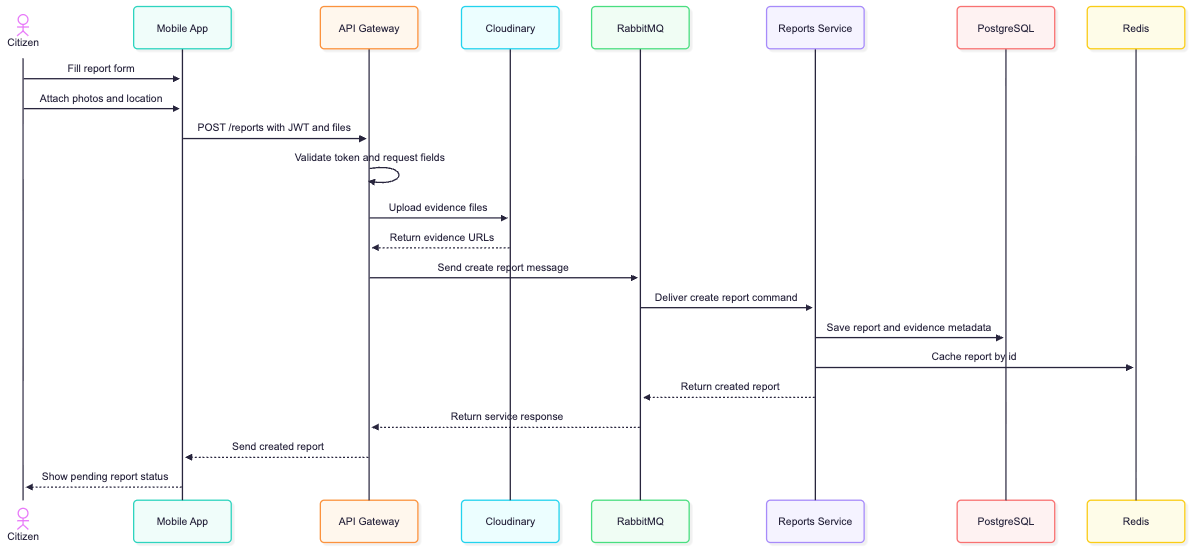
\includegraphics[width=0.9\linewidth,height=0.44\textheight,keepaspectratio]{images/figure3-7-create-report-sequence.png}
    \caption{Sequence of steps from report submission to persistence and cache update.}
    \label{fig:method-create-report-sequence}
\end{figure}

\subsection{Evidence Metadata Handling}

Evidence images are uploaded to Cloudinary rather than stored directly in PostgreSQL \cite{cloudinaryUploadDocs}. The gateway performs the upload and forwards the resulting metadata to the reports service. Storing the Cloudinary public ID alongside the URL makes evidence cleanup possible when reports are deleted. Cloudinary credentials are provided through environment configuration so secrets are not stored in the repository.

\subsection{Review and Status Updates}

Status review is implemented as an administrator-only workflow. Relief users can browse reports, but they do not change status in this thesis version. Administrators update status through the web dashboard; the update request is routed through the gateway to the reports service, which validates the transition, applies the update, and refreshes cached entries.

\section{Client Development Approach}

\subsection{Mobile Client Design}

The mobile client was developed with Expo React Native and TypeScript \cite{expoDocs,reactNativeDocs,typescriptDocs}. The method emphasizes short task completion: sign in, create a report, and view report history. Role-aware navigation is used to present citizen and relief flows without mixing privileged administrator operations into the mobile interface. Redux Toolkit is used to manage authentication state and client-side data flow \cite{reduxToolkitDocs}.

Location entry combines two sources. When permission is granted, the device can provide coordinates. Administrative divisions (province/ward) are selected from the Vietnam Provinces Open API to reduce spelling variation and improve consistency across reports \cite{vietnamProvincesOpenApi}.

\subsection{Dashboard Design}

The web dashboard was developed with Next.js, React, TypeScript, and Tailwind CSS \cite{nextjsDocs,reactDocs,typescriptDocs,tailwindDocs}. It is designed around administrator tasks: triage, evidence inspection, status updates, and user management. The dashboard signs in through the gateway, stores tokens, refreshes sessions when needed, and checks the loaded profile before rendering administrator-only routes.

After authentication, the dashboard loads report lists through the gateway and presents key fields (status, severity, location summary, description) and evidence thumbnails. Filters and search reduce the time required to find relevant cases when many reports arrive close together.

\section{Real-Time Channel Approach}

VietFlood includes a Socket.IO gateway for live location broadcasting \cite{socketioDocs}. A client can emit location updates containing latitude/longitude and optional motion fields. The gateway validates coordinate ranges before rebroadcasting updates to connected clients. Invalid payloads receive an error event. This is treated as a prototype capability to demonstrate real-time communication; operational use would require authentication, clearer authorization rules, and persistent history storage.

\section{Prototype Validation Strategy}

Validation combines two checks: (1) responsibility checks at the code level and (2) scenario walkthroughs across the full stack. Docker Compose is used as the repeatable local environment for backend services and infrastructure dependencies \cite{dockerComposeDocs}.

Scenario walkthroughs focus on whether the prototype supports the intended workflows:
\begin{itemize}
    \item account registration, sign-in, and profile loading;
    \item report creation with location fields and optional photo evidence;
    \item evidence upload and metadata storage;
    \item report listing and detail viewing for citizen, relief, and admin roles;
    \item administrator status updates and cache refresh behavior;
    \item live tracking event broadcast and error handling.
\end{itemize}

These checks are appropriate for a prototype thesis project: they confirm that the system behaves as designed without claiming operational readiness for real disaster response.
